\documentclass[]{article}
\usepackage{lmodern}
\usepackage{amssymb,amsmath}
\usepackage{ifxetex,ifluatex}
\usepackage{fixltx2e} % provides \textsubscript
\ifnum 0\ifxetex 1\fi\ifluatex 1\fi=0 % if pdftex
  \usepackage[T1]{fontenc}
  \usepackage[utf8]{inputenc}
\else % if luatex or xelatex
  \ifxetex
    \usepackage{mathspec}
  \else
    \usepackage{fontspec}
  \fi
  \defaultfontfeatures{Ligatures=TeX,Scale=MatchLowercase}
\fi
% use upquote if available, for straight quotes in verbatim environments
\IfFileExists{upquote.sty}{\usepackage{upquote}}{}
% use microtype if available
\IfFileExists{microtype.sty}{%
\usepackage{microtype}
\UseMicrotypeSet[protrusion]{basicmath} % disable protrusion for tt fonts
}{}
\usepackage[margin=1in]{geometry}
\usepackage{hyperref}
\hypersetup{unicode=true,
            pdftitle={Predicting Gender from Risk-Seeking Behaviors},
            pdfauthor={Deepika Dilip, Rachel Tsong, and Adina Zhang},
            pdfborder={0 0 0},
            breaklinks=true}
\urlstyle{same}  % don't use monospace font for urls
\usepackage{color}
\usepackage{fancyvrb}
\newcommand{\VerbBar}{|}
\newcommand{\VERB}{\Verb[commandchars=\\\{\}]}
\DefineVerbatimEnvironment{Highlighting}{Verbatim}{commandchars=\\\{\}}
% Add ',fontsize=\small' for more characters per line
\usepackage{framed}
\definecolor{shadecolor}{RGB}{248,248,248}
\newenvironment{Shaded}{\begin{snugshade}}{\end{snugshade}}
\newcommand{\KeywordTok}[1]{\textcolor[rgb]{0.13,0.29,0.53}{\textbf{#1}}}
\newcommand{\DataTypeTok}[1]{\textcolor[rgb]{0.13,0.29,0.53}{#1}}
\newcommand{\DecValTok}[1]{\textcolor[rgb]{0.00,0.00,0.81}{#1}}
\newcommand{\BaseNTok}[1]{\textcolor[rgb]{0.00,0.00,0.81}{#1}}
\newcommand{\FloatTok}[1]{\textcolor[rgb]{0.00,0.00,0.81}{#1}}
\newcommand{\ConstantTok}[1]{\textcolor[rgb]{0.00,0.00,0.00}{#1}}
\newcommand{\CharTok}[1]{\textcolor[rgb]{0.31,0.60,0.02}{#1}}
\newcommand{\SpecialCharTok}[1]{\textcolor[rgb]{0.00,0.00,0.00}{#1}}
\newcommand{\StringTok}[1]{\textcolor[rgb]{0.31,0.60,0.02}{#1}}
\newcommand{\VerbatimStringTok}[1]{\textcolor[rgb]{0.31,0.60,0.02}{#1}}
\newcommand{\SpecialStringTok}[1]{\textcolor[rgb]{0.31,0.60,0.02}{#1}}
\newcommand{\ImportTok}[1]{#1}
\newcommand{\CommentTok}[1]{\textcolor[rgb]{0.56,0.35,0.01}{\textit{#1}}}
\newcommand{\DocumentationTok}[1]{\textcolor[rgb]{0.56,0.35,0.01}{\textbf{\textit{#1}}}}
\newcommand{\AnnotationTok}[1]{\textcolor[rgb]{0.56,0.35,0.01}{\textbf{\textit{#1}}}}
\newcommand{\CommentVarTok}[1]{\textcolor[rgb]{0.56,0.35,0.01}{\textbf{\textit{#1}}}}
\newcommand{\OtherTok}[1]{\textcolor[rgb]{0.56,0.35,0.01}{#1}}
\newcommand{\FunctionTok}[1]{\textcolor[rgb]{0.00,0.00,0.00}{#1}}
\newcommand{\VariableTok}[1]{\textcolor[rgb]{0.00,0.00,0.00}{#1}}
\newcommand{\ControlFlowTok}[1]{\textcolor[rgb]{0.13,0.29,0.53}{\textbf{#1}}}
\newcommand{\OperatorTok}[1]{\textcolor[rgb]{0.81,0.36,0.00}{\textbf{#1}}}
\newcommand{\BuiltInTok}[1]{#1}
\newcommand{\ExtensionTok}[1]{#1}
\newcommand{\PreprocessorTok}[1]{\textcolor[rgb]{0.56,0.35,0.01}{\textit{#1}}}
\newcommand{\AttributeTok}[1]{\textcolor[rgb]{0.77,0.63,0.00}{#1}}
\newcommand{\RegionMarkerTok}[1]{#1}
\newcommand{\InformationTok}[1]{\textcolor[rgb]{0.56,0.35,0.01}{\textbf{\textit{#1}}}}
\newcommand{\WarningTok}[1]{\textcolor[rgb]{0.56,0.35,0.01}{\textbf{\textit{#1}}}}
\newcommand{\AlertTok}[1]{\textcolor[rgb]{0.94,0.16,0.16}{#1}}
\newcommand{\ErrorTok}[1]{\textcolor[rgb]{0.64,0.00,0.00}{\textbf{#1}}}
\newcommand{\NormalTok}[1]{#1}
\usepackage{longtable,booktabs}
\usepackage{graphicx,grffile}
\makeatletter
\def\maxwidth{\ifdim\Gin@nat@width>\linewidth\linewidth\else\Gin@nat@width\fi}
\def\maxheight{\ifdim\Gin@nat@height>\textheight\textheight\else\Gin@nat@height\fi}
\makeatother
% Scale images if necessary, so that they will not overflow the page
% margins by default, and it is still possible to overwrite the defaults
% using explicit options in \includegraphics[width, height, ...]{}
\setkeys{Gin}{width=\maxwidth,height=\maxheight,keepaspectratio}
\IfFileExists{parskip.sty}{%
\usepackage{parskip}
}{% else
\setlength{\parindent}{0pt}
\setlength{\parskip}{6pt plus 2pt minus 1pt}
}
\setlength{\emergencystretch}{3em}  % prevent overfull lines
\providecommand{\tightlist}{%
  \setlength{\itemsep}{0pt}\setlength{\parskip}{0pt}}
\setcounter{secnumdepth}{0}
% Redefines (sub)paragraphs to behave more like sections
\ifx\paragraph\undefined\else
\let\oldparagraph\paragraph
\renewcommand{\paragraph}[1]{\oldparagraph{#1}\mbox{}}
\fi
\ifx\subparagraph\undefined\else
\let\oldsubparagraph\subparagraph
\renewcommand{\subparagraph}[1]{\oldsubparagraph{#1}\mbox{}}
\fi

%%% Use protect on footnotes to avoid problems with footnotes in titles
\let\rmarkdownfootnote\footnote%
\def\footnote{\protect\rmarkdownfootnote}

%%% Change title format to be more compact
\usepackage{titling}

% Create subtitle command for use in maketitle
\providecommand{\subtitle}[1]{
  \posttitle{
    \begin{center}\large#1\end{center}
    }
}

\setlength{\droptitle}{-2em}

  \title{Predicting Gender from Risk-Seeking Behaviors}
    \pretitle{\vspace{\droptitle}\centering\huge}
  \posttitle{\par}
    \author{Deepika Dilip, Rachel Tsong, and Adina Zhang}
    \preauthor{\centering\large\emph}
  \postauthor{\par}
      \predate{\centering\large\emph}
  \postdate{\par}
    \date{May 14, 2019}


\begin{document}
\maketitle

\subsection{Introduction}\label{introduction}

One public health phenomenon that has been the subject of debate is the
``Gender and Health Paradox'', in which women experience decreased
quality of life, yet have higher life expectancies than men. A theory
that seeks to explain this pattern outlines increased risk-taking by men
as a causal mechanism. By this logic, men would indicate more
risk-taking behaviors than women when controlled for age and other
confounders. We sought to test this theory by examining if risk-seeking
behaviors could be predictive of gender.

\textbf{Young People's Survey}

For our analysis, we used a data set consisting of 1,010 responses from
a 2013 survey administered among statistics students and their friends
at Comenius University in Bratislava, Slovakia. This dataset is
available to download from Kaggle. The survey consisted of 150 items
including music and movie preferences, hobbies and interests, phobias,
health habits, personality traits, views on life, and opinions, spending
habits, and demographics. Most of the items were presented as a
five-point Likert scale indicating how much a respondent agreed to the
statement. Participants were given the survey in both electronic and
paper formats. To test our hypotheses, we selected 19 variables that
would demonstrate risk-seeking behavior.

After sectioning the data accordingly, we counted missing values to
determine if that could affect our results. When only completed
responses were considered (i.e.~having values for every variable), we
had a sample size of 942; 6.7\% of the data was missing. As this value
was less than 10\%, we decided not to address this via imputation and
opted for a deletion method (complete-case analysis). The limitations of
this method will be addressed in the discussion.

\subsection{Data Exploration}\label{data-exploration}

We checked for collinearity of variables via a correlation matrix; as
there were no significant correlations between any predictors, all of
our original variables were retained. We stratified responses by gender
and visualized them in histograms (fig. 1). Some predictors have more
skewed distributions by gender compared to others (e.g.~cars, war
movies). Other variables such as alcohol use and going outdoors were
more evenly distributed by gender.

We used an unsupervised learning technique (principle component
analysis) to further explore the data (fig.2). Due to the large number
of predictors, the first and second components only explained 17.1\% and
9.4\% of the total variance in the data respectively. Nevertheless, PCA
was insightful in that some of the variables mostly explained by the
first component (interest in cars, adrenaline-driven sports, and active
sports) were skewed toward males.

\textbf{Figure 1}
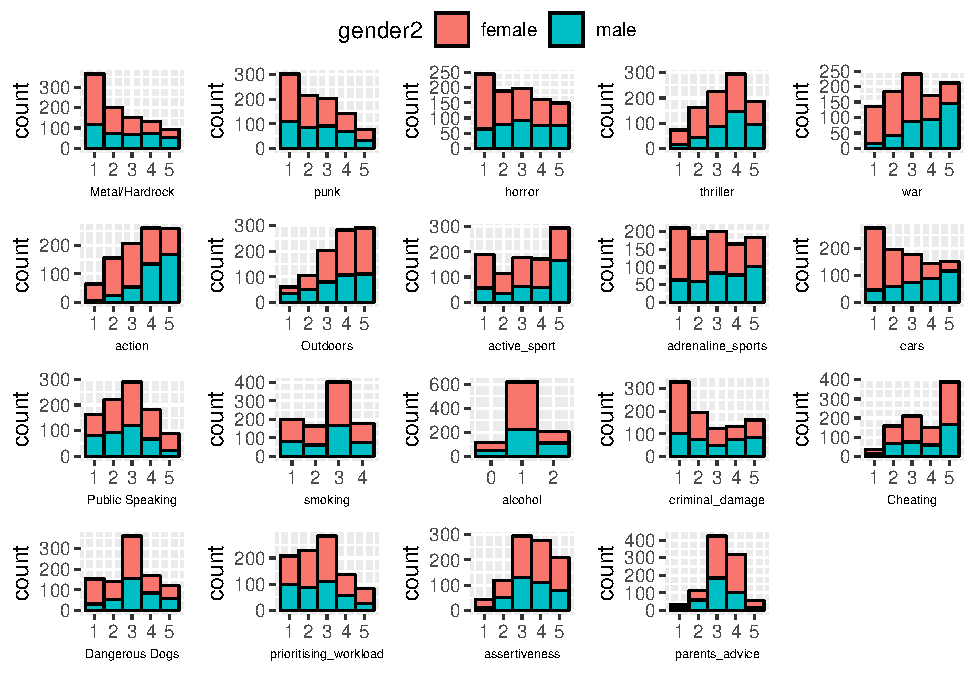
\includegraphics{final_report_files/figure-latex/unnamed-chunk-1-1.pdf}
\textbf{Figure 1}

\begin{verbatim}
##                                  PC1          PC2           PC3
## metal_or_hardrock        0.183335126 -0.305327984  0.6001502593
## punk                     0.135241146 -0.313355525  0.5227974307
## horror                   0.291279074 -0.295250134 -0.1928013131
## thriller                 0.246637978 -0.243706454 -0.0511209522
## war                      0.311653805  0.009247732  0.0932810450
## action                   0.279473794  0.015802676  0.0297065873
## countryside_outdoors     0.002443922  0.285738491  0.1592761068
## active_sport             0.337051025  0.481282425  0.1151283843
## adrenaline_sports        0.390790288  0.295389460  0.0001980147
## cars                     0.394922030  0.192034114 -0.0908512103
## fear_of_public_speaking -0.066643948 -0.154912357  0.0708711106
## smoking                  0.113760888 -0.291594065 -0.3469620527
## alcohol                  0.036069541 -0.073981605 -0.0404212853
## criminal_damage          0.271636665 -0.219261604 -0.1979432755
## cheating_in_school       0.191481747 -0.132673339 -0.2998560809
## small_big_dogs           0.228852618  0.036800532  0.0550586205
## prioritising_workload   -0.067504052  0.173800157  0.0841115161
## assertiveness            0.076323564  0.010849471 -0.0605749892
## parents_advice          -0.039244230  0.111391951  0.0036632908
## gender                   0.107094974  0.002896529  0.0182251776
##                                 PC4          PC5         PC6          PC7
## metal_or_hardrock       -0.16347867  0.023520223 -0.05410151  0.117041904
## punk                    -0.12497717  0.096744995  0.07491989  0.084307996
## horror                   0.43073617  0.312071419  0.39208252 -0.062660821
## thriller                 0.39859643  0.187430207  0.09900111 -0.064445193
## war                      0.20223255 -0.165315625 -0.40991752 -0.026462257
## action                   0.23783881 -0.259800051 -0.21159548 -0.054073094
## countryside_outdoors    -0.00700930  0.029876079  0.06829186 -0.176225873
## active_sport            -0.19145528  0.241278231  0.25493225 -0.024253941
## adrenaline_sports       -0.18246245  0.256587154  0.15838844 -0.132847590
## cars                     0.19500129 -0.258135105 -0.27803890  0.157835751
## fear_of_public_speaking  0.03244770 -0.104604792  0.09994151 -0.584236820
## smoking                 -0.29530647  0.285091258 -0.16500351  0.413088454
## alcohol                 -0.08899757  0.035772294 -0.05319768  0.006118161
## criminal_damage         -0.33372575 -0.656797438  0.47869851 -0.010509355
## cheating_in_school      -0.29344399  0.105191243 -0.19961657 -0.250020561
## small_big_dogs          -0.17923217 -0.003052992 -0.10100039  0.002425578
## prioritising_workload    0.25781108 -0.163726316  0.34191113  0.501137643
## assertiveness           -0.10734112  0.052987530  0.01122002  0.254542960
## parents_advice           0.02895269 -0.019869492  0.04189136  0.044018297
## gender                   0.05605697 -0.072109265 -0.07106180  0.027888758
##                                  PC8         PC9         PC10         PC11
## metal_or_hardrock        0.029573142 -0.04240458  0.088751306  0.003963804
## punk                    -0.115241083  0.23518744  0.059224781 -0.076026200
## horror                   0.118942342 -0.14890020  0.059008517  0.004333842
## thriller                 0.035415236  0.05225906 -0.055103680 -0.050630006
## war                     -0.073849751 -0.48787865 -0.341250892 -0.340618274
## action                   0.034991254  0.30864702 -0.020150743 -0.077962260
## countryside_outdoors    -0.171206206 -0.40537255  0.505683127 -0.416165442
## active_sport            -0.125153924  0.21103257 -0.553452399 -0.104168023
## adrenaline_sports       -0.008299503 -0.05222342  0.328311147  0.135861515
## cars                    -0.213189372  0.29190604  0.339506151  0.256440011
## fear_of_public_speaking -0.503186817  0.07770446  0.018397101  0.217605180
## smoking                 -0.528932140 -0.12981250 -0.020349816 -0.013374541
## alcohol                 -0.032567548 -0.03600096 -0.016564021  0.049884133
## criminal_damage          0.043777961 -0.10365739 -0.052733551 -0.127136423
## cheating_in_school       0.037141831  0.16912593  0.127136991 -0.240882402
## small_big_dogs           0.274322457 -0.42217127 -0.027812231  0.633235089
## prioritising_workload   -0.293066703 -0.09066029  0.067008972  0.058823594
## assertiveness            0.398023898  0.19227420  0.229233667 -0.261963465
## parents_advice          -0.127718862  0.02871235  0.007604438 -0.060091932
## gender                   0.008525452  0.01115334 -0.048168113  0.019199207
##                                PC12         PC13        PC14         PC15
## metal_or_hardrock        0.09877146  0.165731058 -0.14126656 -0.118252329
## punk                    -0.05063396 -0.092789090  0.27436086  0.020726192
## horror                   0.10571337  0.232467524  0.02821330 -0.048102650
## thriller                 0.03200745 -0.199711837 -0.14419195 -0.043269863
## war                     -0.09576475  0.046217494  0.24903993  0.313714791
## action                  -0.10013332 -0.569184648 -0.34238523 -0.206447038
## countryside_outdoors     0.20871428 -0.004402493 -0.30019333 -0.218369292
## active_sport             0.23261894  0.129644040 -0.15755471 -0.042092638
## adrenaline_sports       -0.58237732 -0.198700682  0.21711451  0.160802116
## cars                     0.12214484  0.481522211  0.03907988 -0.017742937
## fear_of_public_speaking  0.17726412 -0.059290776 -0.11439749  0.477869654
## smoking                 -0.07548460 -0.082053075 -0.29852055  0.005887646
## alcohol                 -0.04511377 -0.011293940  0.01986171  0.019395395
## criminal_damage         -0.09731201  0.064600523 -0.05679713 -0.053124521
## cheating_in_school       0.44751932 -0.174202066  0.49569939 -0.194493364
## small_big_dogs           0.35582028 -0.250858814 -0.08774969  0.001684453
## prioritising_workload    0.24728543 -0.326577890  0.35531011  0.073656977
## assertiveness            0.21975243 -0.045619837 -0.23034868  0.698534052
## parents_advice           0.13094032 -0.192106518  0.02857588  0.035253989
## gender                  -0.04933097  0.047466435 -0.03109024 -0.026329773
##                                PC16          PC17         PC18
## metal_or_hardrock        0.31071076 -0.5320547263  0.073388573
## punk                    -0.31021604  0.5310430047 -0.162972989
## horror                  -0.27231703 -0.2030461002 -0.355643342
## thriller                 0.49470773  0.3628484867  0.467502038
## war                     -0.01816037  0.0003051455 -0.035566854
## action                  -0.27465206 -0.2128138207 -0.151169575
## countryside_outdoors    -0.11570823  0.1801461049  0.042903657
## active_sport            -0.05365054  0.0034494119  0.043253927
## adrenaline_sports        0.11542154 -0.1453726813  0.038786581
## cars                     0.04920777  0.1414752858 -0.003316439
## fear_of_public_speaking -0.04414658 -0.1214740602  0.042968185
## smoking                 -0.05850801  0.0006815067 -0.022031339
## alcohol                 -0.03945589  0.0293978213 -0.022456457
## criminal_damage          0.07462692  0.0956303979  0.013767160
## cheating_in_school       0.03720193 -0.1576146596  0.094377043
## small_big_dogs          -0.07844585  0.1911673923 -0.047721230
## prioritising_workload   -0.06159237 -0.2103008448  0.208773242
## assertiveness           -0.04078425 -0.0062254393  0.014242927
## parents_advice           0.59499804  0.1054200797 -0.731801737
## gender                  -0.03229904 -0.0398720743  0.011687209
##                                 PC19          PC20
## metal_or_hardrock        0.013623083 -4.643184e-02
## punk                    -0.047788189  2.566019e-02
## horror                   0.001160956 -1.485730e-02
## thriller                 0.033000726 -2.106925e-05
## war                     -0.037879805 -7.998898e-02
## action                   0.010983174 -9.213318e-02
## countryside_outdoors     0.055146473  4.080400e-02
## active_sport             0.028590589 -2.466699e-02
## adrenaline_sports       -0.038194455  7.775743e-03
## cars                     0.002650659 -9.625004e-02
## fear_of_public_speaking -0.008445835  3.591659e-02
## smoking                 -0.111311016  1.431953e-02
## alcohol                  0.979547728 -9.503765e-02
## criminal_damage         -0.015048577 -2.259836e-02
## cheating_in_school      -0.021872229  4.836056e-02
## small_big_dogs          -0.058538772  3.848582e-03
## prioritising_workload    0.058278888  1.767951e-02
## assertiveness            0.022382941  2.803471e-02
## parents_advice           0.027057130  5.287475e-02
## gender                   0.093936236  9.763168e-01
\end{verbatim}

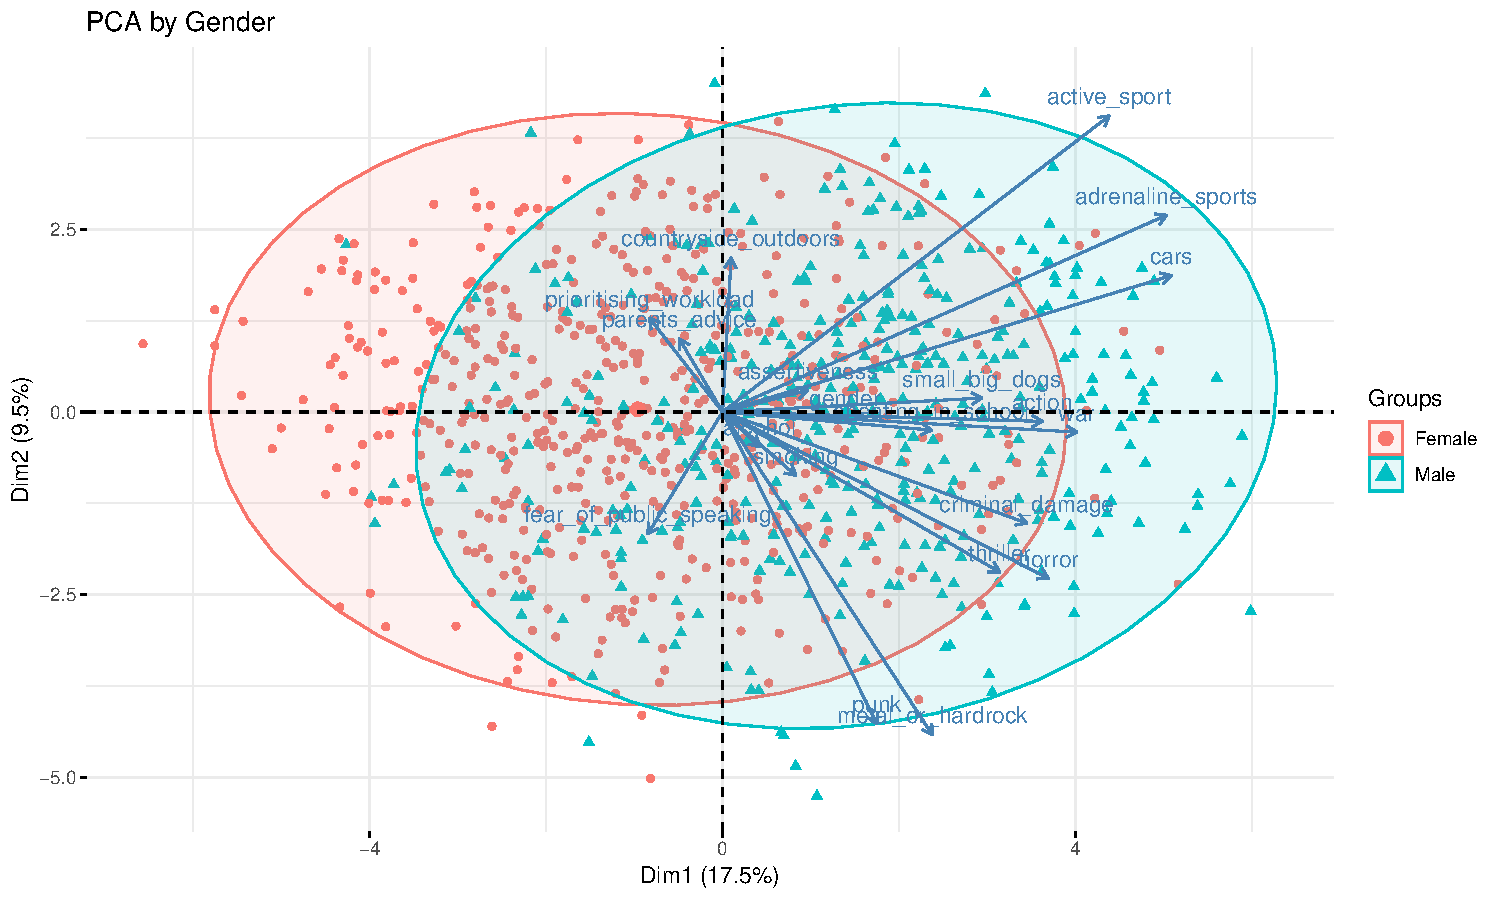
\includegraphics{final_report_files/figure-latex/unnamed-chunk-2-1.pdf}
\textbf{Figure 2}

\subsection{Method}\label{method}

We selected 19 variables that were related to thrill or risk seeking
behaviors. The following variables were included in our analysis:

\begin{itemize}
\tightlist
\item
  Interest in: (ranked 1-5 from ``don't enjoy at all'' to ``enjoy very
  much'')
\item
  Metal, hard rock music
\item
  Punk music
\item
  Horror movies
\item
  War movies
\item
  Action movies
\item
  Outdoor activities
\item
  Sport at a competitive level
\item
  Adrenaline sports
\item
  Cars
\item
  Fears of public speaking (ranked 1-5 from ``not afraid at all'' to
  ``very afraid of'')
\item
  Smoking habits (categorical with 4 levels: ``never smoked'', ``tried
  smoking'', ``former smoker'', ``current smoker'')
\item
  Drinking habits (categorical with 3 levels: ``never'', ``social
  drinker'', ``drink a lot'')
\item
  Statements about personality traits: (ranked 1-5 from ``strongly
  disagree'' to ``strongly agree'')
\item
  I damaged things in the past when I get angry
\item
  I used to cheat at school
\item
  I prefer big dangerous dogs to smaller, calmer dogs
\item
  I try to do tasks as soon as possible and not leave them until last
  minute
\item
  I'm not afraid to give my opinion if I feel strongly about something
\item
  I always listen to my parents' advice
\end{itemize}

Variables that were ranked on a scale from 1-5 were considered as
continous responses. After splitting the data into training and testing
sets using an 80/20 split, we fit the following models to the training
data:

\begin{itemize}
\tightlist
\item
  Logistic regression
\item
  Discriminant analysis (linear and quadratic)
\item
  KNN
\item
  Support vector machine (linear and radial kernels)
\item
  Classification trees (random forest and boosting)
\end{itemize}

Training and test error were calculated for each model to evaluate
overfitting. The final models was chosen by assessing the training data
using the \texttt{resamples()} function in the \texttt{caret} package.

\subsection{Models}\label{models}

\subsubsection{Logistic Regression}\label{logistic-regression}

Logistic regression assumes independent observations, a sufficiently
large sample size, and a linear relationship between the predictors and
the log-odds of the outcome. As we used simple logistic regression, it
does not contain any tuning parameters. When examining the predictor
parameters, the following ones had a p-value of less than 0.001:
\texttt{cars}, \texttt{war}, \texttt{action}, and
\texttt{metal\_or\_hardrock}.

\subsubsection{Discriminant Analysis}\label{discriminant-analysis}

\textbf{Linear}

Linear discriminant analysis assumes normally distributed features. LDA
does not contain any tuning parameters and is strong when considering
more than 2 predictors. Additionally, it works well when the classes are
well separated and Gaussian distribution assumptions are applied. When
ranking variables (using the function \texttt{varImp()}), the most
important ones were as follows: \texttt{cars}, \texttt{war},
\texttt{action}, \texttt{active\_sport}, and \texttt{thriller}.

\textbf{Quadratic}

Just like LDA, QDA works well when the classes are well separated and
Gaussian distribution (normally -distributed) assumptions are applied.
However, unlike LDA, it assumes that each class has its own covariance
matrix. QDA does not contain any tuning parameters. When ranking
variables (using the function varImp()), the most important ones were as
follows: \texttt{cars}, \texttt{war}, \texttt{action},
\texttt{active\_sport}, and \texttt{thriller}.

\subsubsection{KNN}\label{knn}

The method of K-nearest neighbors makes no assumptions about the shape
of the decision boundary; therefore, if the decision boundary is highly
non-linear then this model will perform better than others. This model
has one tuning parameter, K, the number of closest training points. An
optimal value of K was chosen by repeated cross-validation using the
\texttt{train()} function in the \texttt{caret} package by specifying
the tuning grid. One drawback of this model is that we cannot assess
variable importance.

\subsubsection{SVM}\label{svm}

\textbf{Linear}

The support vector classifier has one tuning parameter, C. Using the
\texttt{train()} function in the \texttt{caret} package the best C was
0.0433, which was chosen by cross-validation. Since the support vector
classifier is a hyperplane, the model assumes that the decision boundary
is linear, which is a potential drawback if the decision boundary is
non-linear.

\textbf{Radial}

The support vector machine with a radial kernel has two tuning
parameters. One is C, the cost parameter, and the other is the degree of
non-linearity sigma. We used the \texttt{train()} function in the
\texttt{caret} package to choose these parameters by cross-validation.
The best C was 78.033 and the best sigma was 0.000335. This model
assumes a non-linear boundary. One potential drawback of support vector
machines is that you cannot assess variable importance or estimate
probabilities as in logistic regression.

\subsubsection{Random Forest}\label{random-forest}

A Random Forest (RF) model was fit with the \texttt{caret} package using
the \texttt{ranger} method. We chose Random Forest as one of our models
because it is an ensemble method for classification trees that uses a
collection of models to improve the final prediction. Random Forest was
also chosen over bagging as an esemble method because it minimizes
correlation between the decisions trees that are grown. In our model,
500 decision trees were grown and the gini index was selected as a
splitrule. The minimum number of variables to randomly sample at each
split (mtry) and minimum node size were tuned using repeated
cross-validation in the \texttt{caret} packages with ROC as the measure
of performance. The best tuning results were \texttt{mtry\ =\ 2} and
\texttt{min.node.size\ =\ 6}. According to the final model, the most
important variables for classification are \texttt{cars},
\texttt{action}, and \texttt{war}.

\subsubsection{Extreme Gradient
Boosting}\label{extreme-gradient-boosting}

An Extreme Gradient Boosting (XGB) model was fit using the
\texttt{xgboost} packages in \texttt{caret}. Gradient Boosting is
another ensemble method for classification trees. It differs from other
ensemble methods such as random forest because the algorithm focuses on
modelling errors from previous models in order to improve the
bias-variance tradeoff. We selected the \texttt{xgboost} package and
algorithm because it performs more efficiently than the \texttt{gbm}
package discussed in class. Multiple parameters were tuned using
repeated cross-validation with ROC as the unit of measurement. The final
model selected \texttt{nrounds\ =\ 100}, \texttt{max\_depth\ =\ 2},
\texttt{eta\ =\ 0.1}, \texttt{colsample\_bytree\ =\ 0.8}. The final
model showed that \texttt{cars}, \texttt{action}, and \texttt{war} were
the most important variables for classifying gender.

\begin{Shaded}
\begin{Highlighting}[]
\CommentTok{# List of models}
\NormalTok{models =}\StringTok{ }\KeywordTok{list}\NormalTok{(log.fit, lda.fit, qda.fit, knn.fit, }
\NormalTok{              svm_linear, svm_radial, rf.fit, xgb.fit)}

\CommentTok{# Function which will succinctly summarize confusion matrix results in table format (although specified for test data also works with training data)}
\NormalTok{test_summary =}\StringTok{ }\ControlFlowTok{function}\NormalTok{(data, model)\{}
  \CommentTok{# Fit predictions using specified model}
\NormalTok{  pred =}\StringTok{ }\KeywordTok{predict}\NormalTok{(model, }\DataTypeTok{newdata =}\NormalTok{ data)}
  
  \CommentTok{# Confusion Matrix}
\NormalTok{  test_matrix =}\StringTok{ }\KeywordTok{confusionMatrix}\NormalTok{(}\DataTypeTok{data =}\NormalTok{ pred,}
                \DataTypeTok{reference =} \KeywordTok{factor}\NormalTok{(data}\OperatorTok{$}\NormalTok{gender),}
                \DataTypeTok{positive =} \StringTok{"male"}\NormalTok{)}
  
  \CommentTok{# First join table}
\NormalTok{  join1 =}\StringTok{ }\NormalTok{test_matrix}\OperatorTok{$}\NormalTok{overall }\OperatorTok\StringTok{ }\KeywordTok{tibble}\NormalTok{() }\OperatorTok\StringTok{ }
\StringTok{    }\KeywordTok{rename}\NormalTok{(}\StringTok{"Test"}\NormalTok{ =}\StringTok{ "."}\NormalTok{) }\OperatorTok\StringTok{ }
\StringTok{    }\KeywordTok{mutate}\NormalTok{(}\DataTypeTok{Measure =} \KeywordTok{c}\NormalTok{(}\StringTok{"Accuracy"}\NormalTok{, }\StringTok{"Kappa"}\NormalTok{, }\StringTok{"AccuracyLower"}\NormalTok{, }\StringTok{"AccuracyUpper"}\NormalTok{,}
                     \StringTok{"AccuracyNull"}\NormalTok{, }\StringTok{"AccuracyPValue"}\NormalTok{, }\StringTok{"McnemarPValue"}\NormalTok{)) }\OperatorTok\StringTok{ }
\StringTok{    }\KeywordTok{spread}\NormalTok{(}\DataTypeTok{key =}\NormalTok{ Measure, }\DataTypeTok{value =}\NormalTok{ Test) }\OperatorTok\StringTok{ }
\StringTok{    }\KeywordTok{mutate}\NormalTok{(}\DataTypeTok{TestError =} \DecValTok{1} \OperatorTok{-}\StringTok{ }\NormalTok{Accuracy) }\OperatorTok\StringTok{ }
\StringTok{    }\KeywordTok{select}\NormalTok{(Accuracy, TestError)}

  \KeywordTok{return}\NormalTok{(join1)}
\NormalTok{\}}
\end{Highlighting}
\end{Shaded}

\begin{longtable}[]{@{}lrr@{}}
\toprule
Models & TrainError & TestError\tabularnewline
\midrule
\endhead
Logistic & 0.2066225 & 0.2032086\tabularnewline
LDA & 0.2119205 & 0.1925134\tabularnewline
QDA & 0.1523179 & 0.2085561\tabularnewline
KNN & 0.2291391 & 0.2139037\tabularnewline
SVM Linear & 0.2092715 & 0.1818182\tabularnewline
SVM Radial & 0.2039735 & 0.1871658\tabularnewline
Random Forest & 0.0000000 & 0.1764706\tabularnewline
XGBoost & 0.1562914 & 0.1764706\tabularnewline
\bottomrule
\end{longtable}

Table 1: Testing and training error rates among eight classification
models

\subsection{Model Selection}\label{model-selection}

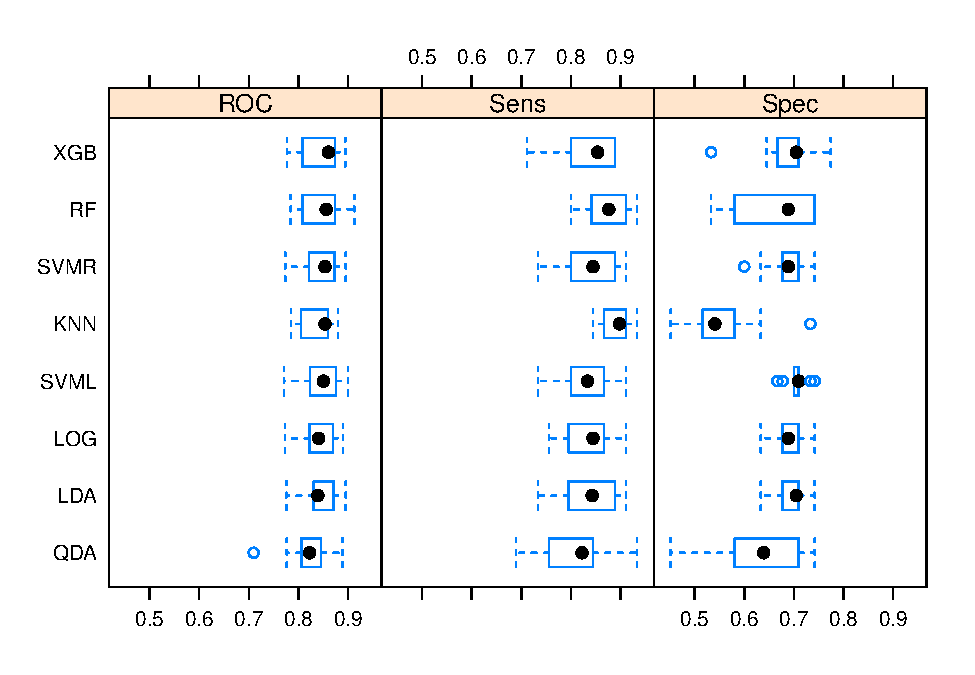
\includegraphics{final_report_files/figure-latex/unnamed-chunk-13-1.pdf}

\subsection{Final Model}\label{final-model}

Based off of our resampling results through the \texttt{caret} package,
the best model to predict gender was the XGBoost model. The most
important variables for classification are \texttt{cars},
\texttt{action}, and \texttt{war}. A classification tree by itself is
very easy to interpret, however the use of ensemble methods utilizes
multiple trees making a final model more difficult to visualize or
interpret.

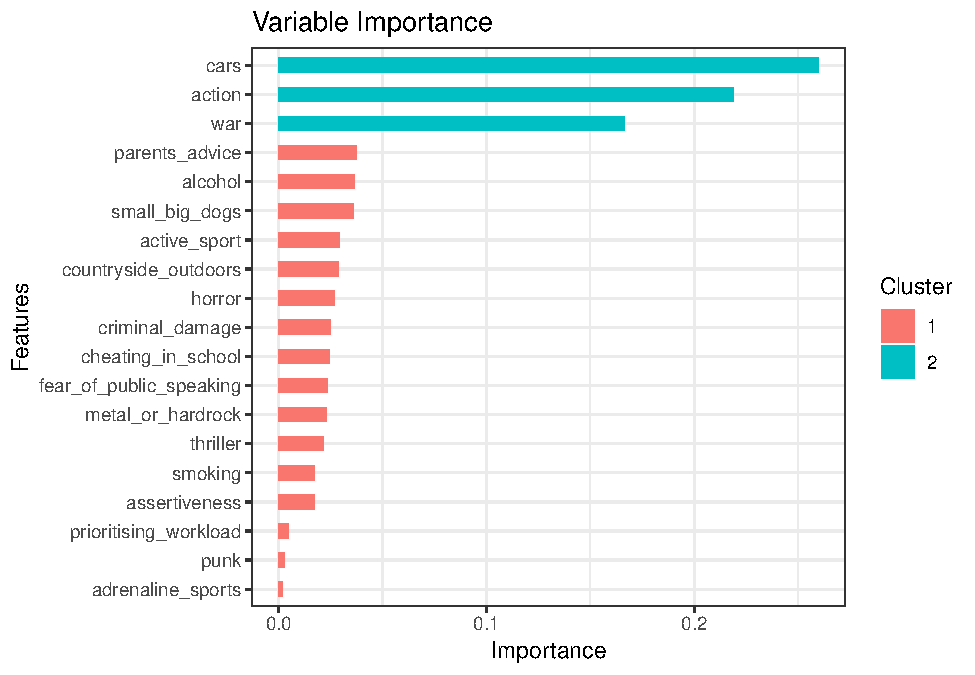
\includegraphics{final_report_files/figure-latex/unnamed-chunk-14-1.pdf}

\subsection{Conclusion}\label{conclusion}

Some of the limitations of this report include translation issues. The
original language of the survey was Slovakian, and this could influence
interpretations. Additionally, this affects generalizability of findings
as the population of this survey was specifically statistics students in
Slovakia. The deletion method used would also present issues if data
were not missing at random, resulting in bias.

\newpage

\subsection{Appendix}\label{appendix}


\end{document}
